%==============================================================================
\chapter{Metodologia}\label{desenvolvimento}
%==============================================================================

Neste capítulo será explicado o método proposto para resolver o problema de \ac{pos} Tagging, onde primeiramente será definida as técnicas utilizadas para seu funcionamento.

Com a intuição de simplificar o entendimento, já definimos variáveis que serão utilizadas no método de aprendizagem. Elas podem ser encontradas na \autoref{tab:variaveisdesenvolvimento}.

\begin{table}[!htb]
\caption{Notação utilizada para o treinamento do modelo} \label{tab:variaveisdesenvolvimento}
\begin{center}
\begin{tabular}{m{2cm}m{12.0cm}}
  \toprule
  $d$		& dimensão das palavras vetorizadas \\
  $t$		& tamanho da janela de palavras \\
  $\omega$	& conjunto de palavras \\
  $\gamma$  & conjunto de classes gramaticais \\
  $c_i^t$  & sequência de classes gramaticais que começa em $i$ e termina em $t$ \\
  $w_i^t$  & sequência de palavras que começa em $i$ e termina em $t$ \\
  $c_i$		& i-ésima classe gramatical \\
  $z_i$		& i-ésima classe vetorizada com dimensão $d$ \\ 
  $w_i$		& i-ésima palavra\\
  $v_i$		& i-ésima palavra vetorizada com dimensão $d$ \\
  $V_i$		& vetor centrado em $i$ com as $t$ palavras vetorizadas concatenadas \\
  $s_c(V_i)$ & pontuação de uma sequência $V_i$ ter a classe gramatical $c$ \\
  $A_{c,d,e}$ & pontuação de ir de uma classe $c$, passar por $d$ e chegar a $e$ \\
  $Q$	&	conjunto com os índices das palavras vetorizadas já classificadas \\
  \bottomrule
\end{tabular}
\end{center}

\end{table}



\section{Representação das palavras}

Seguimos a ideia explorada em massa pela literatura de representar as palavras através de vetores reais com uma dimensão fixa $d$ definida pelo usuário. Isso será feito utilizando três estratégias já mencionadas: \ac{nlm}, \ac{sg} e \ac{glove}. Ou seja, para cada $w_i \in \omega$, geramos o vetor $v_i \in \mathbb{R}^d $.

Além das \textit{word embeddings}, utilizaremos outras duas \textit{features} importantes no contexto de \ac{pos} Tagging, como capitalização que consegue, na maioria das vezes, distinguir nomeações, e também prefixos, que podem ser usadas para distinguir medidas de tempo, velocidade, etc. 

Em ordem de manter a rede neural homogênea, também iremos transformar cada classe gramatical em um vetor. Com isso poderemos aplicar funções que combinam características do vetor de uma palavra com o vetor de uma classe gramatical.


\section{Pontuações para estrutura gramatical}

Para classificar palavras em uma sentença, o etiquetador obtém uma janela de palavras de tamanho fixo a cada momento, e transforma as palavras em vetores de \textit{features}, que são então passadas para uma rede neural descrita em \cite{collobert2008unified}. A rede atribui para cada classe gramatical $c \in \gamma$ uma pontuação. A etapa de gerar pontuações para a palavra ocorre no mesmo momento que o treinamento do modelo. A saída para toda a sentença é então passada para o algoritmo de Viterbi \cite{viterbi1967error}, que realiza uma predição estruturada em um tempo polinomial.

Seguimos a estratégia apresentada em \cite{dos2014training} para realizar as pontuações. Nela, a ideia é de que a classe gramatical de uma palavra depende fortemente das palavras vizinhas, o que é verdade para várias aplicações de \ac{pln}, incluindo \ac{pos} Tagging.

Dada uma janela com $t$ palavras $\{w_1, w_2, ..., w_t\}$, que foram transformadas para sua representação vetorial $\{v_1, v_2, ..., v_t\}$, para computar a n-ésima palavra, é centralizada a janela em $n$ e concatena-se todas as palavras da metade à esquerda e da metade à direita em um novo vetor $V_n$ de dimensão $t * d$. Para palavras no começo ou no fim da sentença, é usado vetores com valores fixos para preencher o espaço vazio na janela de palavras. A \autoref{eq:janeladevets} demonstra isso.

\begin{equation} \label{eq:janeladevets}
V_n = \big\{ v_{n - (t-1)/2}, ..., v_n, ..., v_{{n + (t-1)/2}} \big\}
\end{equation}

Seguimos \cite{fonseca2015evaluating} e computamos a pontuação $s_c(V_n)$ para cada classe gramatical $c$ da palavra no meio da janela. 


Além disso, usamos a ideia apresentada em \cite{collobert2011natural}, onde é feito um esquema de predição que leva em consideração a estrutura gramatical. O método usa uma pontuação de transição $A_{c,d}$, inicializada com 0, para ir de uma classe $c \in \gamma$ para uma classe $d \in \gamma$ conforme a sequência das palavras. Porém extendemos a notação para funcionar com trigramas: $A_{c,d,e}$. A estrutura $A$ consegue armazenar informações importantes como ``após um pronome é bastante provável que há um verbo''. Depois que a rede produz a pontuação para todas as palavras, a pontuação final de uma sequência de classes gramaticais $c_1^t$ para uma sequência de palavras $w_1^t$, é dada pela \autoref{eq:pontuacaofinal}. $Q$ representa um conjunto com os índices das palavras que já foram classificadas.

\begin{equation} \label{eq:pontuacaofinal}
S(w_1^t, c_1^t) = \sum\limits_{k=1}^{t} \Big( \argmax_{1 \leq i \leq t, v_i \notin Q} (s_{c_i}(V_i) + A_{c_{i-1}, c_{i}, c_{i+1}}) \Big)
\end{equation}

Após computar isso para cada palavra na sentença, a classe gramatical final é prevista através do algoritmo de Viterbi.


\section{Treinamento}

Realizamos um treinamento supervisionado utilizando uma rede neural recursiva para a classificação das palavras em suas respectivas classes gramaticais. O modelo completo da rede neural pode ser visto na \autoref{fig:neuralnetworkfinal}.

\begin{figure}[htb]
    \caption{Modelo da rede neural}\label{fig:neuralnetworkfinal}
    \begin{center}
        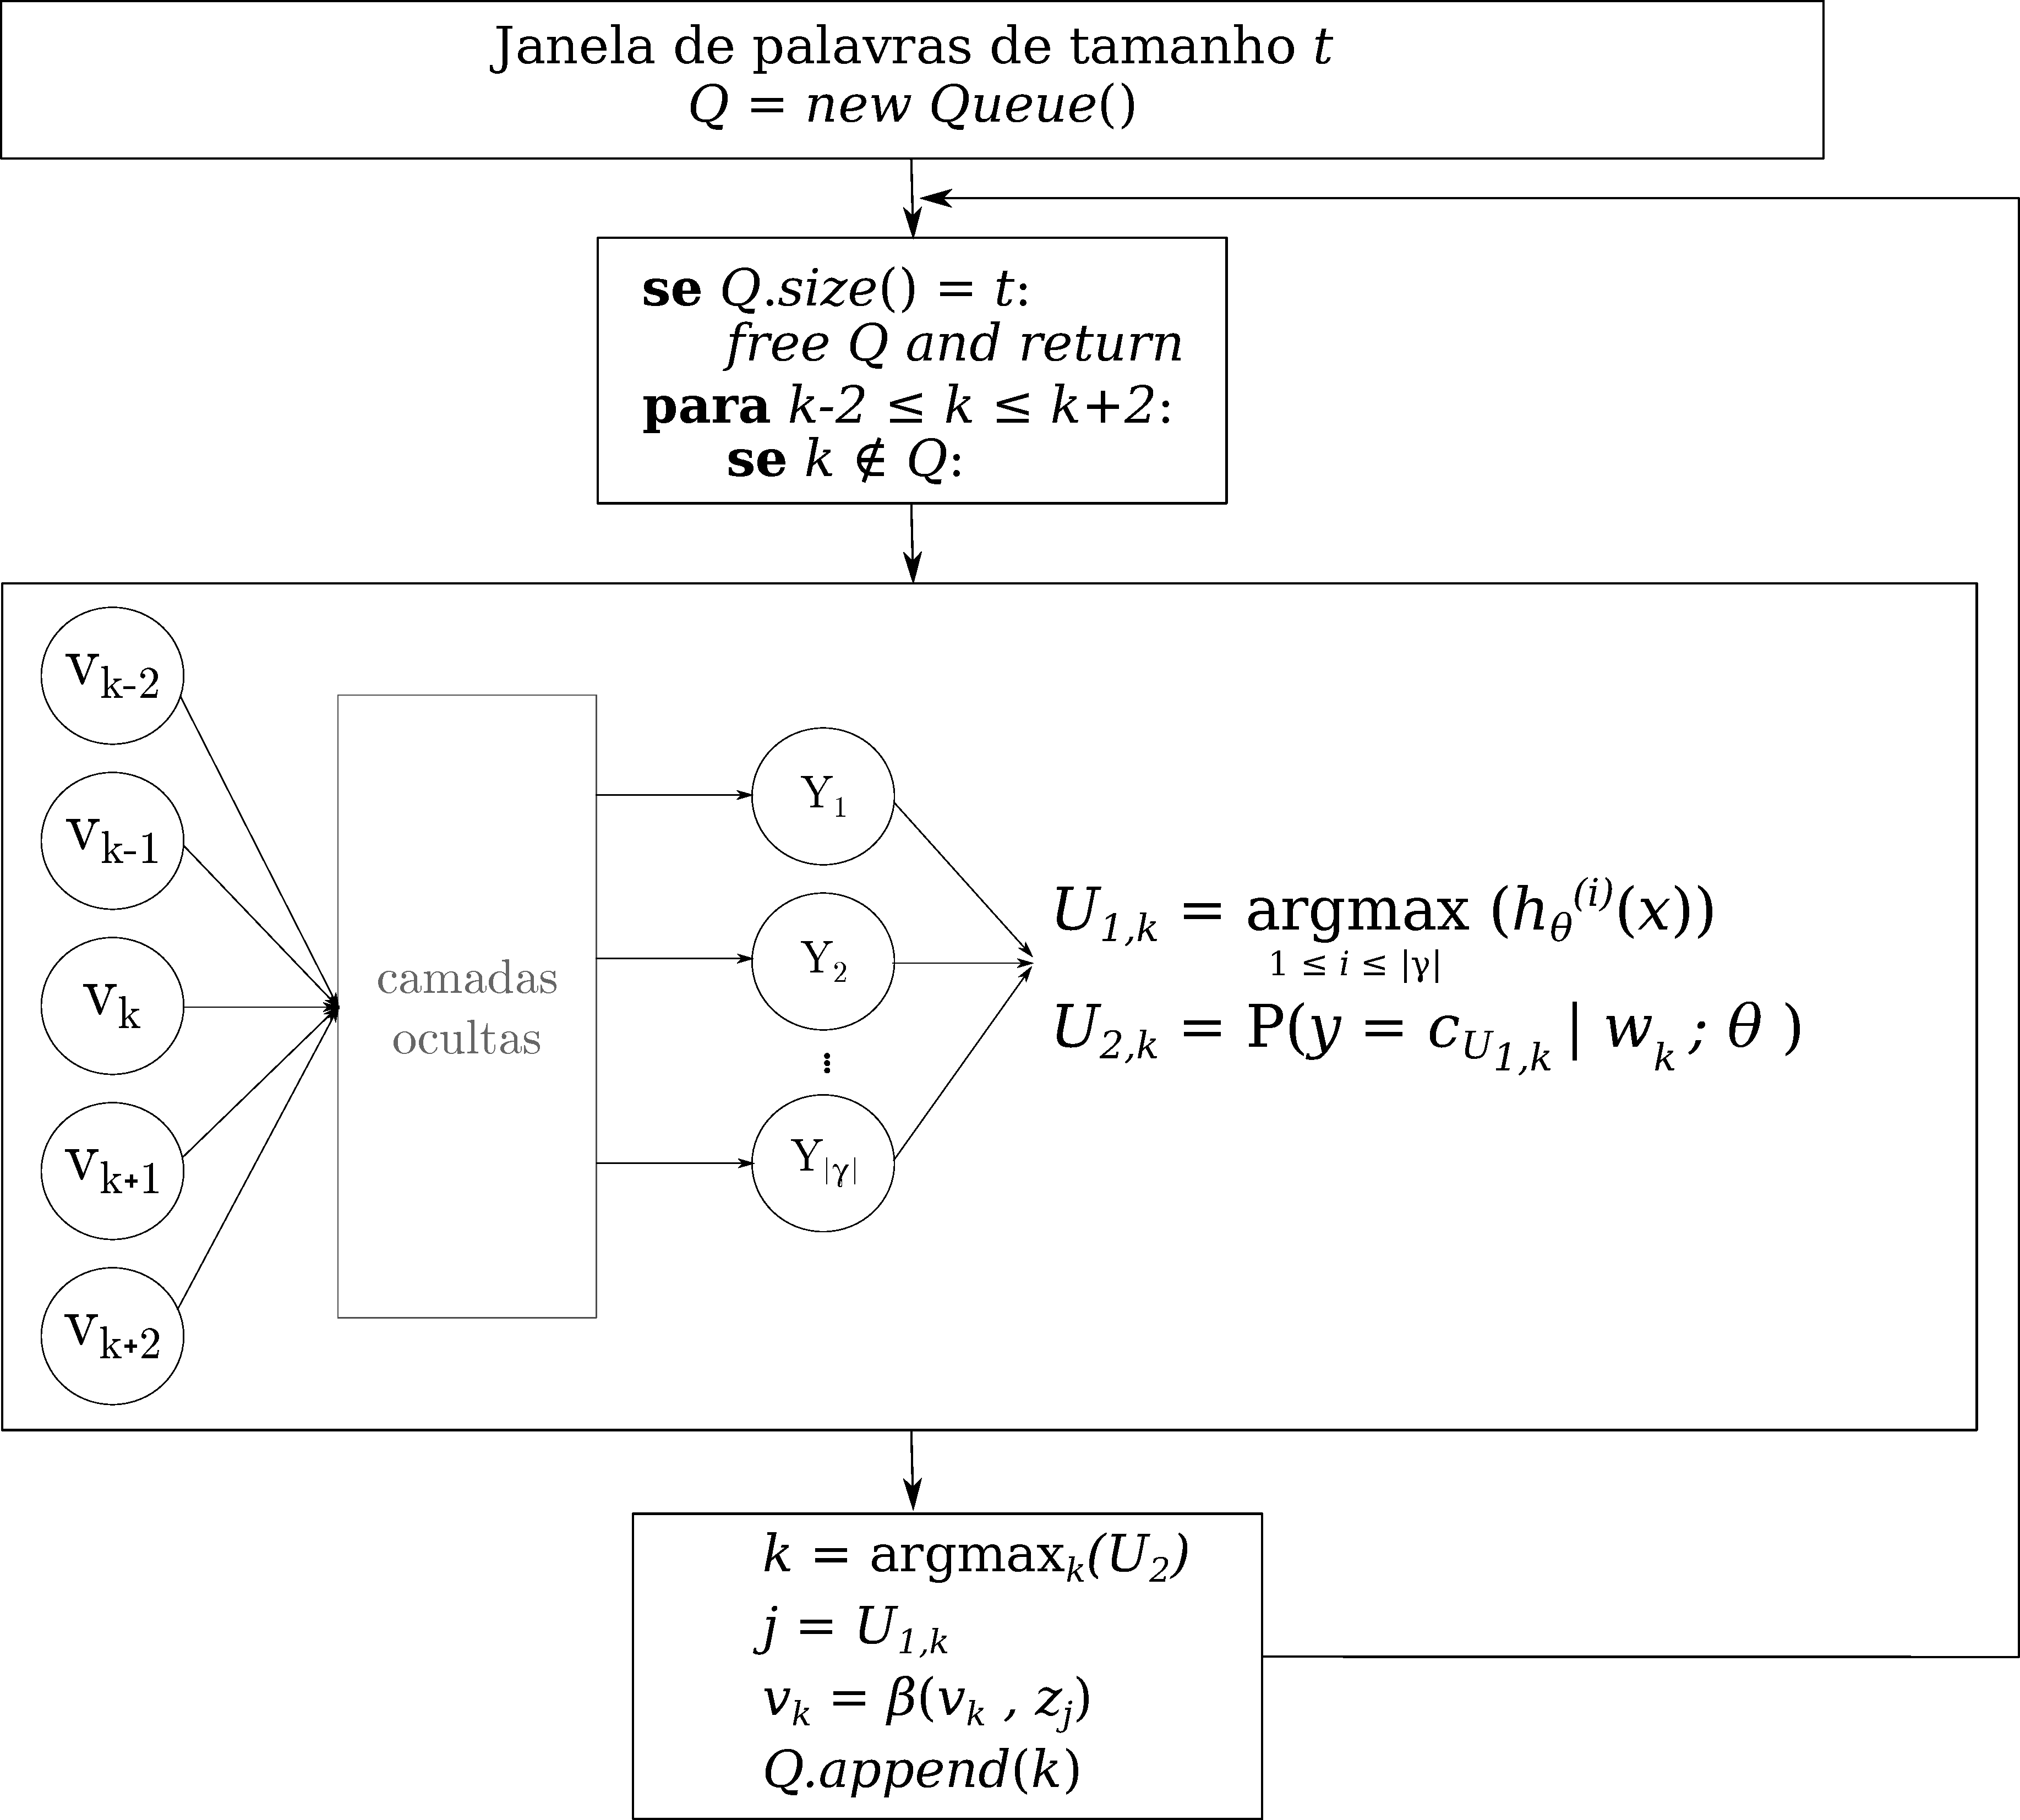
\includegraphics[scale=0.25]{img/neuralnetworkfinal_alg2.pdf}
    \end{center}
\end{figure}

Para treinar a rede neural, será seguido uma estratégia de aprendizagem guiada por palavras mais fáceis \cite{shen2007guided}. A \autoref{fig:guidedlearning} exemplifica transições mais fáceis em uma frase, onde o peso mais baixo na aresta representa a ordem de execução. Na verdade, cada transição de um nodo para outro conta como uma nova etapa de treinamento. A \autoref{eq:pontuacaofinal} faz esse aprendizado guiado ao realizar a escolha da palavra mais fácil através da maximização das possibilidades que ainda não foram testadas dentro da janela de palavras.

\begin{figure}[htb]
	  \caption{Grafo de transições de palavras mais fáceis}\label{fig:guidedlearning}
	  \begin{center}
	      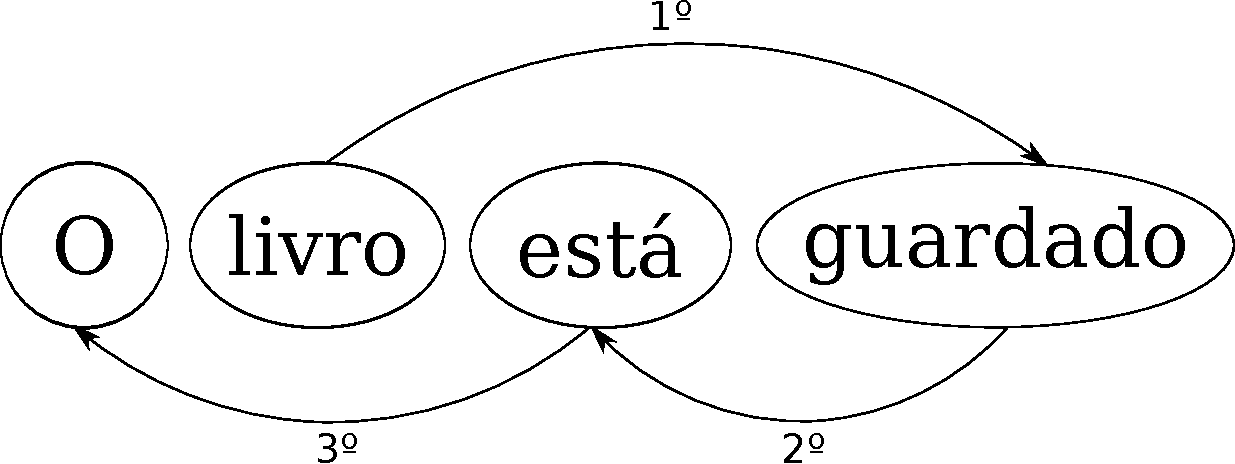
\includegraphics[scale=0.3]{img/guidedlearning.pdf}
	  \end{center}
\end{figure}

Treinar o modelo consiste em ajustar os pesos da rede neural, os valores das \textit{word embeddings} e as pontuações de transição. Após descobrir qual a classe gramatical mais provável para uma palavra $w_n$, o vetor da classe gramatical $z_c$ é composto com o vetor da própria palavra $v_n$ através de uma operação de soma. Essa composição é então armazenada no vetor da própria palavra, conforme mostrado abaixo. 

\begin{equation} \label{eq:composicaovets}
v_n = v_n + z_n
\end{equation}

Na rede neural da \autoref{fig:neuralnetworkfinal}, as camadas ocultas foram removidas da imagem para simplificar a visualização. A saída da rede neural é armazenada num conjunto temporário $U$, que tem duas listas. A primeira lista tem os índices da classe preditada para a palavra sendo analisada $w_k$, já a segunda lista contém as probabilidades da classe preditada ser da palavra $w_k$. Após isso, recupera-se qual a palavra que tem a maior probabilidade de ser classificada. O vetor da classe da palavra recuperada $z_j$ é composto com o vetor da palavra analisada $v_j$ através da \autoref{eq:composicaovets} e o processo se repete até que o conjunto $Q$ tenha tamanho $t$.

Para treinar a rede neural, todos os ajustamentos são feitos em ordem de maximizar a seguinte equação:

\begin{equation}
\sum\limits_{(w_1^t,c_1^t) \in \phi} P(c_1^t|w_1^t,\theta) \nonumber \\
\end{equation}

Onde $\phi$ denota o conjunto dos pares de palavras e classes gramaticais. Computamos a probabilidade acima utilizando uma operação \textit{softmax} \cite{Bengio-et-al-2015-Book}:

\begin{align}
P(c_1^t|w_1^t,\theta) = &\ \dfrac{e^{S(w_1^t, c_1^t)}}{\sum\limits_{u_1^t \in \gamma^t} e^{S(w_1^t, u_1^t)}} \nonumber \nonumber \\
log(P(c_1^t|w_1^t,\theta)) = &\ S(w_1^t, c_1^t) - log\Bigg(\sum\limits_{u_1^t \in \gamma^t} e^{S(w_1^t, u_1^t)} \Bigg) \nonumber
\end{align}

A função de custo pode ser definida como:

\begin{equation} \label{eq:costfunctionfinalnn}
J(\theta) = log\Bigg(\sum\limits_{u_1^t \in \gamma^t} e^{S(w_1^t, u_1^t)} \Bigg) - S(w_1^t, c_1^t)
\end{equation}

Onde, há princípio, ajustamos os pesos $\theta$ da rede utilizando o Gradiente Descendente sobre o primeiro termo da função de custo, porém vamos testar com outros algoritmos mais eficientes para essa tarefa, como o Gradiente Descendente Estocástico, Adagrad, Adadelta, etc. \cite{Bengio-et-al-2015-Book}. 

Também queremos maximizar o segundo termo da \autoref{eq:costfunctionfinalnn}. Para isso, seguimos \cite{fonseca2015evaluating} e realizamos um incremento nas pontuações de transição para cada palavra etiquetada em cada etapa do \textit{Backpropagation}, conforme mostrado na equação abaixo:

\begin{equation}\label{eq:gradientsfinalnn}
\frac{\partial J(\theta)}{\partial A_{c_{i-1}, c_{i}, c_{i+1}}} \text{ += } 1 \quad \forall i
\end{equation}


Além disso, incrementamos a função $s_c(v_k) \text{ += } 1$, onde $v_k$ representa a palavra no meio da janela sendo analisada.